%%
% BIThesis 研究生学位论文模板 The BIThesis Template for Graduate Thesis
% This file has no copyright assigned and is placed in the Public Domain.
%%

\chapter{相关工作}
\label{chap:related-work}

\begin{figure}[H]
  \centering
  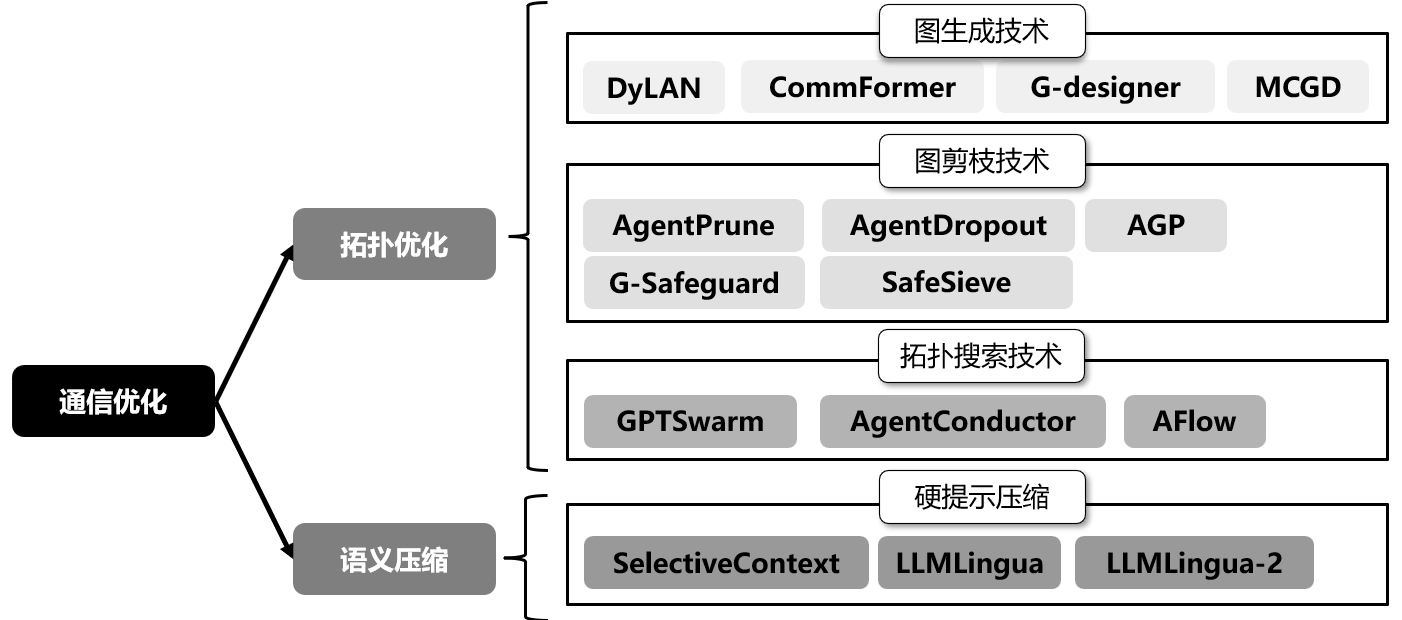
\includegraphics[width=0.65\textwidth]{image/第一章/图 1‑3：多智能体的两条研究路线.png}
  \caption{多智能体的两条研究路线}
  \label{fig:related_work_routes}
\end{figure}

为了应对多智能体系统中日益凸显的通信瓶颈，近年来学术界与工业界在通信机制优化方面进行了大量探索。依据优化对象的不同，现有研究主要可以分为两类：一类关注智能体协作的组织方式与通信路径，核心问题是“哪些智能体之间需要通信”；另一类关注通信路径上传递的自然语言内容，核心问题是“通信时应传递什么信息”。本章首先介绍多智能体系统的基本范式，随后分别围绕语义冗余问题和通信边冗余问题梳理相关研究，为后续两项工作提供研究脉络。

\section{多智能体系统}

多智能体系统（Multi-Agent Systems，MAS）通常由多个具备不同角色、能力或工具权限的智能体组成，各智能体通过通信、协商、验证和分工协作共同完成复杂任务。与单智能体方法相比，MAS能够引入多视角推理和交叉验证机制，使系统在软件开发、复杂问答、数学推理和开放环境交互等任务上表现出更强的任务拆解能力与鲁棒性\cite{ref9,ref31,ref35,ref36}。

现有大语言模型多智能体系统大多围绕角色分工和通信机制展开。ChatDev\cite{ref9}将软件开发流程拆解为多个具有明确职责的智能体，并通过阶段化对话完成需求分析、编码和测试；MetaGPT\cite{ref35}引入标准化操作程序，将产品经理、架构师、工程师等角色组织为结构化流水线；AutoGen\cite{ref36}则提供灵活的对话式多智能体编程框架，使不同智能体可以根据任务需要进行自由组网和交互。这些工作说明，多智能体系统的性能不仅取决于单个基座模型的能力，还取决于角色设置、通信拓扑、历史记忆和工具使用方式。

从通信结构看，MAS常见拓扑包括完全连接、链式、层状、星状和二分图拓扑等\cite{ref37}。完全连接拓扑有利于信息充分共享，但通信边数会随智能体数量呈平方级增长；链式或层状拓扑能够控制传递路径，但可能限制跨角色的信息互补；星状拓扑依赖中心智能体完成调度和汇总，易形成瓶颈。随着任务轮次增加和工具观察写入上下文，静态拓扑和全量消息传递会进一步放大Token消耗，并导致关键信息被冗余历史淹没。因此，后续研究逐渐从两个层面优化MAS通信：一是压缩通信内容，解决语义冗余问题；二是优化通信路径，解决通信边冗余问题。


\section{语义冗余问题}

\subsection{定义和分类}

除了在通信拓扑层面减少冗余交互外，在语义维度直接对智能体传递的上下文消息进行压缩，是降低大型语言模型（LLMs）推理成本、提升内存利用率的另一项重要手段。与拓扑优化关注“哪些智能体之间需要通信”不同，语义冗余问题更关注“沿通信链路传递什么内容”。在多智能体系统中，语义冗余通常指智能体之间传递的自然语言消息中包含大量重复推理、弱相关背景、低价值解释或过长历史记忆，使下游智能体需要在更长上下文中寻找真正有用的信息。

结合多智能体通信过程，语义冗余主要可以分为三类。第一类是\textbf{角色不匹配冗余}，即发送方完整推理并不完全符合接收方智能体的角色职责，导致下游节点接收大量与自身任务无关的信息。第二类是\textbf{多前驱重复冗余}，即多个上游智能体围绕同一事实、同一公式或同一候选答案给出相似表述，增加上下文长度但信息增量有限。第三类是\textbf{跨轮历史冗余}，即多轮协作中历史消息逐轮累积，使后续智能体难以从冗长上下文中定位当前共识、关键分歧和有效证据。

\begin{figure}[H]
  \centering
  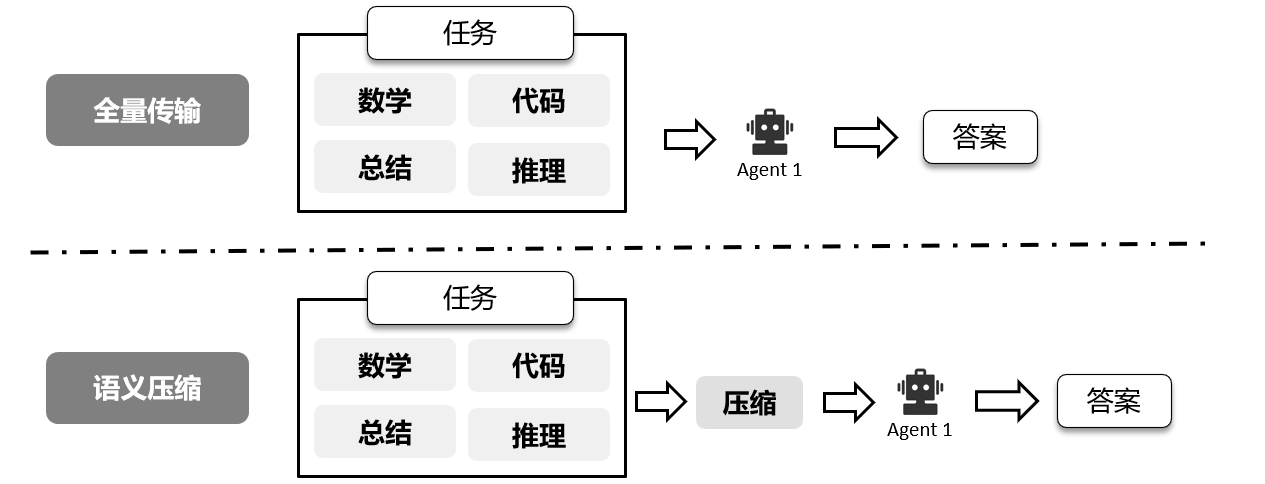
\includegraphics[width=0.65\textwidth]{image/第一章/图1-7：压缩示意图.png}
  \caption{压缩示意图}
  \label{fig:prompt_compression}
\end{figure}

\subsection{通用应对策略}

硬提示词压缩旨在通过对原始文本进行修改，生成人类可读的、更为精简的自然语言序列。与软提示压缩将上下文映射为不可读的连续向量不同，硬提示词压缩保留了自然语言形式，因此更便于人工检查、跨模型迁移以及在多智能体通信场景中复用。根据压缩机制的不同，主流研究主要可划分为以下两个方向\cite{ref54}：

\par\indent \textbf{基于过滤的压缩方法：}
此类方法通过评估词元、短语或句子的重要性，剔除冗余和低信息量的部分，并在保持原文顺序的基础上生成压缩后的上下文。早期代表性工作SelectiveContext\cite{ref55}利用较小规模的因果语言模型计算词元的自信息或困惑度，将低自信息内容视为更容易由上下文预测、因而冗余度更高的部分，再按照词元、短语或句子粒度进行过滤。该方法无需额外训练，能够直接应用于黑盒LLM，但由于其重要性评估主要依赖语言统计特征，可能误删对特定任务有用但语言上并不突出的信息。LLMLingua\cite{ref56}进一步提出粗到细的压缩框架，首先通过预算控制器在指令、示例和问题等不同提示词组成部分之间分配压缩率，再利用小模型估计词元困惑度或信息熵，逐步保留高信息量词元。相比简单过滤，LLMLingua考虑了提示词内部不同模块的重要性差异，并通过迭代式压缩缓解局部删除造成的上下文断裂问题，因此能够在较高压缩率下保持较好的下游任务性能。

    后续的LLMLingua-2\cite{ref57}则引入了数据蒸馏机制，将压缩任务从基于困惑度的无监督筛选转化为词元级二分类任务。具体而言，该方法先利用强模型生成抽取式压缩结果，再通过自动对齐为原始文本中的词元标注“保留”或“删除”标签，并训练轻量级双向编码器预测每个词元的重要性。推理时，模型按照保留概率选择满足压缩预算的词元，并保持其原始顺序。由于双向编码器能够同时利用左右上下文，LLMLingua-2在压缩速度、忠实度和跨任务泛化方面均优于单纯依赖困惑度的方法。进一步地，TACO-RL\cite{ref58}将强化学习引入过滤式压缩过程，将每个词元的保留或删除视为动作，并根据下游任务表现给予奖励。例如，在问答任务中可依据答案F1值评估压缩效果，在摘要任务中可依据生成文本与参考文本的相似度计算奖励。通过这种方式，TACO-RL能够根据具体任务目标动态调整剪枝策略，使压缩器更倾向于保留与当前查询或任务评价指标直接相关的信息，从而弥补任务无关过滤方法在语义选择上的不足。

\par\indent \textbf{基于重写的压缩方法：}
与简单的删除词元不同，此类方法利用语言模型强大的生成与概括能力，主动将冗长的上下文重写为更紧凑的自然语言表达。其核心优势在于能够跨越句子边界进行信息重组，将分散在原文不同位置的关键信息合并为更短的表述，从而避免纯过滤方法可能造成的语义割裂或可读性下降。例如Nano-Capsulator框架\cite{ref59}不再直接从原始提示词中选择词元，而是训练一个生成式压缩模型，将长提示词封装为更短的Capsule Prompt。该模型在训练过程中同时考虑语义保持和下游任务效用：一方面要求压缩后的自然语言表示尽可能保留原始提示词的核心含义，另一方面又通过目标LLM在相关任务上的输出表现约束压缩结果，使其不仅短，而且仍然能够有效引导模型完成任务。

    与过滤式方法相比，基于重写的压缩能够生成更加流畅、连贯且人类可读的压缩文本，尤其适合处理包含重复解释、长链式推理示例或多轮对话历史的上下文。在多智能体系统中，这类方法可用于将某一智能体的长篇推理过程、观察记录或工具调用结果重写为面向后续智能体的短摘要，从而减少跨智能体传递的词元数量。然而，这类方法也存在一定风险：由于压缩过程依赖生成模型，可能出现关键信息遗漏、语义偏移甚至幻觉。因此，在高精度任务中，重写式压缩通常需要结合任务反馈、事实一致性检测或保守的压缩率设置，以在压缩效率与语义可靠性之间取得平衡。

\section{通信边冗余问题}

\subsection{定义和分类}

通信边冗余问题是指多智能体系统中存在大量低价值、重复或成本过高的信息传递路径，使系统在没有获得相应任务收益的情况下产生额外Token消耗、工具调用开销和上下文膨胀。与语义冗余关注单条消息内部内容不同，通信边冗余关注“哪些边应当存在、哪些边应当被削弱或剪除”。在工具调用场景中，该问题更加突出，因为一条通信边不仅传递发送方的自然语言推理，还可能传播搜索结果、代码执行结果和文本检查结果等高成本工具观察。

通信边冗余主要可以分为三类。第一类是\textbf{空间边冗余}，即同一轮内过密的智能体连接使多个下游节点读取相似或低贡献的上游输出。第二类是\textbf{时间边冗余}，即跨轮历史状态被机械传递，导致早期低价值信息在多轮推理中持续占用上下文。第三类是\textbf{工具传播冗余}，即外部工具返回的长观察结果沿通信边反复传播，进一步放大模型输入Token、工具Token和推理成本。

\subsection{通用应对策略}

针对通信边冗余，现有方法通常将智能体视为节点、通信链路视为边，并通过图生成、图剪枝和拓扑搜索等方式减少低价值通信路径\cite{ref38}。这类方法的共同目标是在保持协作收益的同时，使信息只沿更有贡献的边传播。

\par\indent \textbf{基于图生成的策略：}
图生成方法旨在根据任务条件自适应构造通信拓扑，而不是完全依赖人工预设结构。
\begin{figure}[H]
  \centering
  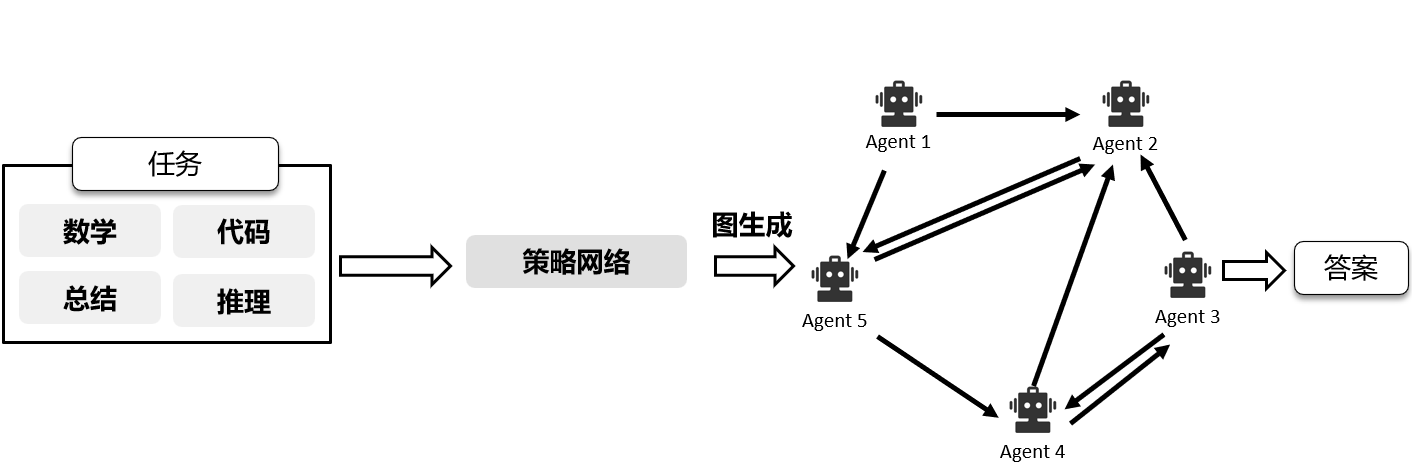
\includegraphics[width=0.65\textwidth]{image/第一章/图1-4：图生成技术.png}
  \caption{图生成技术示意图}
  \label{fig:graph_generation}
\end{figure}

DyLAN（Dynamic LLM-Agent Network）\cite{ref39}并不预先固定所有智能体之间的通信关系，而是将多智能体协作过程建模为随任务推进变化的前馈式动态网络。其核心机制包括两个阶段：首先在候选智能体集合中进行团队优化，利用Agent Importance Score评估不同智能体在当前任务上的边际贡献；随后在任务求解阶段，根据每一轮智能体输出的有效性动态选择后续参与通信的节点。DyLAN还引入早停机制，当系统已经形成足够稳定的答案或共识时提前终止多轮交互。因此，它降低成本的方式不是压缩单条消息，而是减少低贡献智能体的参与次数、削减无效讨论轮次，并动态生成更贴合当前查询的通信图。

CommFormer\cite{ref40}将多智能体强化学习中的智能体表示为图节点，将通信信道表示为有向边，并通过可微的图结构学习机制直接优化通信拓扑。其关键做法是对离散边选择进行连续松弛，使邻接矩阵能够参与梯度更新，同时在Transformer结构中引入关系增强注意力，以建模智能体间的依赖关系。G-Designer\cite{ref41}面向LLM多智能体系统，将每个智能体的基础模型、角色、状态、工具插件等编码为节点特征，并额外引入任务虚拟节点来表达当前查询需求，随后使用变分图自编码器生成面向特定任务的通信图。MCGD\cite{ref42}则从多智能体强化学习角度构建稀疏协调图，通过图扩散模型学习有效交互模式，体现了只显式建模关键邻居关系、避免全体智能体两两交互的思路。

\par\indent \textbf{基于图剪枝的策略：}
图剪枝方法通常从密集拓扑出发，逐步删除低贡献节点或通信边，使原本冗余的通信图收敛为更稀疏的协作结构。
\begin{figure}[H]
  \centering
  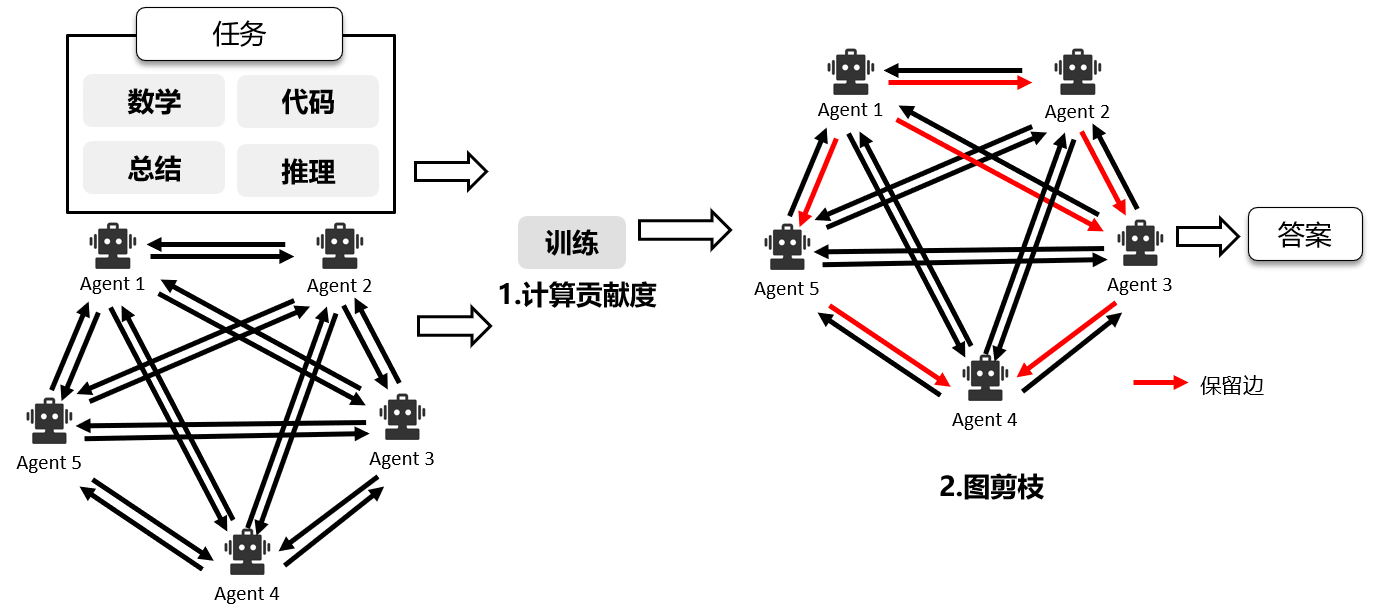
\includegraphics[width=0.65\textwidth]{image/第一章/图1-5：图剪枝技术.png}
  \caption{图剪枝技术示意图}
  \label{fig:graph_pruning}
\end{figure}

AgentPrune\cite{ref43}将LLM多智能体系统表示为空间-时间通信图：同一轮智能体之间的信息交换为“空间边”，跨轮历史传递为“时间边”。它为这些边学习可剪枝的图掩码，并通过系统效用评估器判断不同边对任务结果的贡献。由于外部LLM调用和任务评估通常不可微，AgentPrune使用策略梯度近似优化掩码参数，并最终执行一次性硬剪枝。AgentDropout\cite{ref44}在边剪枝基础上进一步引入节点丢弃，通过Node Dropout和Edge Dropout同时减少智能体输入、输出和后续通信边。SafeSieve\cite{ref45}采用渐进式软剪枝策略，结合LLM语义评估、角色互补性和历史任务表现修正边权，并利用聚类机制保持核心功能簇连通性。AGP（Adaptive Graph Pruning）\cite{ref46}同时进行节点级硬剪枝和边级软剪枝，使系统能够针对不同查询生成不同规模的稀疏拓扑。G-Safeguard\cite{ref47}则从安全角度构建multi-agent utterance graph，用于识别异常节点与异常话语，并通过隔离风险节点或剪断高风险外发边阻止恶意信息扩散。

\par\indent \textbf{基于拓扑搜索的策略：}
拓扑搜索通过在智能体算子和通信边构成的庞大空间中探索高效工作流，通常结合强化学习、蒙特卡洛树搜索或网络架构搜索算法。
\begin{figure}[H]
  \centering
  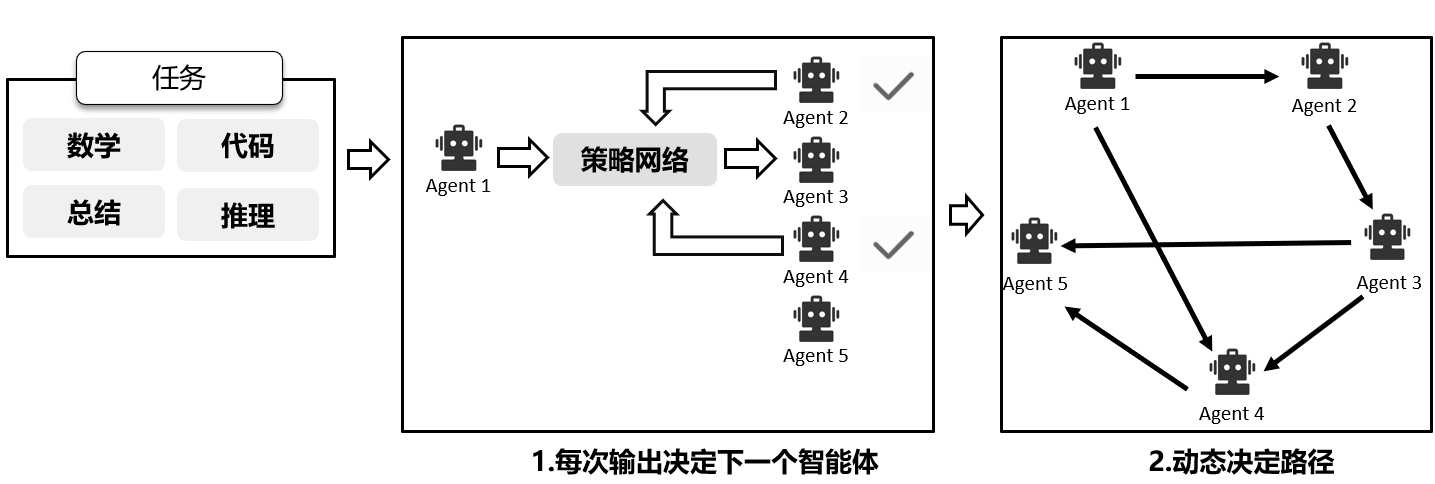
\includegraphics[width=0.65\textwidth]{image/第一章/图1-6：拓扑搜索技术.png}
  \caption{拓扑搜索技术示意图}
  \label{fig:topology_search_related}
\end{figure}

GPTSwarm\cite{ref48}将语言智能体系统统一建模为可优化图：节点可以是LLM调用、工具或数据处理函数，边表示信息流。它为候选边分配可学习的采样概率，在无环图空间中采样候选拓扑，并通过REINFORCE等策略梯度方法根据任务效用更新边概率。AgentConductor\cite{ref49}面向竞赛级代码生成任务，训练LLM为每个问题动态生成YAML格式的分层DAG拓扑，并根据编译、运行和测试反馈多轮调整拓扑。AFlow\cite{ref50}将agentic workflow表示为可执行代码中的算子组合与依赖关系，并使用蒙特卡洛树搜索探索Generate、Review、Revise、Ensemble、Test、Programmer等工作流算子。MASS（Multi-Agent System Search）\cite{ref51}交错优化prompt和topology，并对低收益模块进行影响力剪枝。MaAS（Multi-agent Architecture Search via Agentic Supernet）\cite{ref52}提出智能体超网，使每个查询只激活少量算子路径。DynaSwarm\cite{ref53}则在GPTSwarm式参数化通信图基础上引入样本级动态选择，根据输入样本路由到不同稀疏候选结构。

上述研究说明，减少无效节点、无效边和低收益工作流能够显著缓解多智能体系统的通信负担。但现有方法大多将通信边代价近似视为同质，或者主要依据任务效用判断边是否保留，对工具调用场景中“某条边传播了多少工具观察、触发了多少下游上下文膨胀、带来了多少额外调用成本”刻画不足。尤其在搜索、代码执行和文本检查等工具增强任务中，一条边的价值不仅取决于是否提高最终答案，还取决于它是否传播了高成本、低增益的工具信息。因此，本文第四章提出面向通信边冗余的图剪枝算法，将通信边建模为可学习概率，并把任务正确性、工具调用次数、工具返回Token和模型输出Token共同纳入边级优化目标，从而解决工具调用场景下通信边价值异质、成本难以归因和低贡献边难以及时剪除的问题。

\section{本章小结}

本章围绕多智能体系统及其通信效率优化相关研究进行了梳理。首先，多智能体系统通过角色分工、协作推理和工具调用提升复杂任务处理能力，但也带来了通信路径膨胀和上下文累积问题。其次，语义冗余问题主要表现为角色不匹配、多前驱重复和跨轮历史冗余，现有过滤式与重写式压缩方法为减少自然语言上下文提供了基础，但仍需面向多智能体通信场景进一步适配。最后，通信边冗余问题主要表现为空间边、时间边和工具传播冗余，现有图生成、图剪枝和拓扑搜索方法能够从结构层面降低系统开销，但对工具调用场景下的边级成本归因、工具观察传播和动态低价值边识别仍不充分。上述不足共同构成了本文后续两个工作的主要动机：第三章从语义内容层面提出面向语义冗余的消息压缩框架，第四章从通信结构层面提出面向通信边冗余的图剪枝算法。
